\section{Design of a Robust DC-NET Variant}

\begin{frame}{DC-NET Robustness Problems}
    
    \begin{alertblock}{Cheating}
        Malicious participants send incorrect values in their output messages.
    \end{alertblock}
    
    \begin{alertblock}{Collision}
        More than one participant send a message in their output messages.
    \end{alertblock}
    
\end{frame}

\begin{frame}{Real Round - Key-Sharing}
    \begin{columns}[c]
        \column{.5\textwidth}
            \hspace{-0.9cm}
            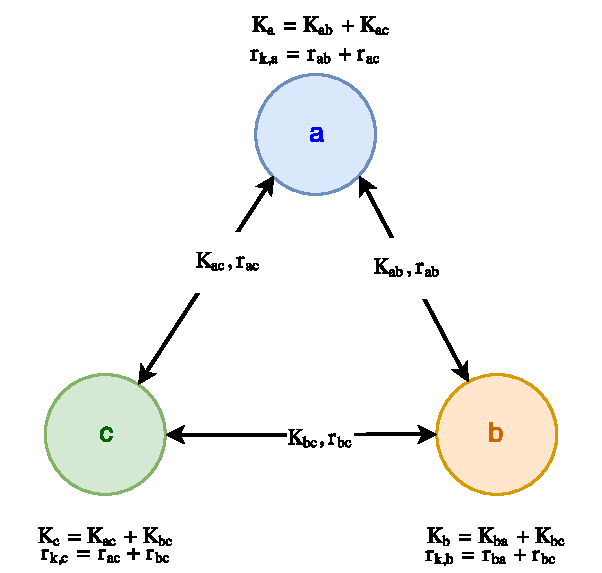
\includegraphics[scale=.6]{images/keys-sharing.pdf}
            \vspace{.2cm}
            \setbeamercolor{postit}{fg=black,bg=yellow}
            \centering
            \begin{beamercolorbox}[sep=.5em,wd=3cm,center]{postit}
                $K_{ij} = -K_{ji}$\\
                $r_{ij} = -r_{ji}$
            \end{beamercolorbox}
        \column{.5\textwidth}
            \begin{block}<2->{Commitments on Keys}
                    \centering
                    \includegraphics<2-2>[scale=0.5]{images/commitment.png}
                    \only<3>
                    {\centering
                    $c_{k,a} = g^{K_a} h^{r_{k,a}}$\\
                    $c_{k,b} = g^{K_b} h^{r_{k,b}}$\\
                    $c_{k,c} = g^{K_c} h^{r_{k,c}}$}
            \end{block}
            \begin{block}<2->{PoK on Keys}
                \centering
                \includegraphics<2-2>[scale=0.5]{images/pok.png}
                \only<3>
                {\centering
                \scriptsize$\mathtt{PoK}_{k,a} = PoK\{(K_a, r_{k,a}): c_{k,a} = g^{K_a} h^{r_{k,a}}\}$\\
                \scriptsize$\mathtt{PoK}_{k,b} = PoK\{(K_b, r_{k,b}): c_{k,b} = g^{K_b} h^{r_{k,b}}\}$\\
                \scriptsize$\mathtt{PoK}_{k,c} = PoK\{(K_c, r_{k,c}): c_{k,c} = g^{K_c} h^{r_{k,c}}\}$\\}
            \end{block}
            \begin{exampleblock}<3->{Check values}
                \centering
                $\prod c_{k,i} \overset{?}{=} 1$
            \end{exampleblock}
    \end{columns}
\end{frame}